\documentclass[tikz]{standalone}

\begin{document}
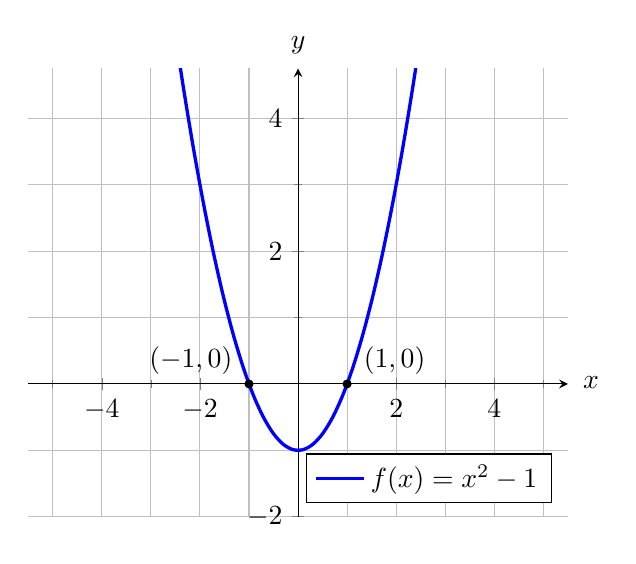
\begin{tikzpicture}
    \begin{axis}[%
        xlabel=$x$, ylabel=$y$, legend pos=south east,
        grid=both, xmin=-5.5, xmax=5.5, ymin=-2, ymax=4.75,
        axis lines = middle,
        minor x tick num=1, minor y tick num=1,
        xlabel style = {at={(axis description cs:1.01,0.3)},anchor=west},
        ylabel style = {at={(axis description cs:0.5,1.01)},anchor=south},
    ]
    \addplot[blue, very thick, domain=-5:5, smooth, samples=50] plot {x^2-1};
    \filldraw[black] (-1,0) circle (.5mm) node[above left,xshift=-2.5pt]{$(-1,0)$}
    	(1,0) circle (.5mm) node[above right,xshift=2.5pt]{$(1,0)$};
    \legend{$f(x)=x^2-1$}
    \end{axis}
\end{tikzpicture}
\end{document}
